\let\negmedspace\undefined
\let\negthickspace\undefined
\documentclass[journal]{IEEEtran}
\usepackage[a5paper, margin=10mm, onecolumn]{geometry}
%\usepackage{lmodern} % Ensure lmodern is loaded for pdflatex
\usepackage{tfrupee} % Include tfrupee package

\setlength{\headheight}{1cm} % Set the height of the header box
\setlength{\headsep}{0mm}     % Set the distance between the header box and the top of the text

\usepackage{gvv-book}
\usepackage{gvv}
\usepackage{algorithmicx} % Ensure algorithmicx is loaded explicitly
\usepackage{cite}
\usepackage{amsmath,amssymb,amsfonts,amsthm}
\usepackage{graphicx}
\usepackage{textcomp}
\usepackage{xcolor}
\usepackage{txfonts}
\usepackage{listings}
\usepackage{enumitem}
\usepackage{mathtools}
\usepackage{gensymb}
\usepackage{comment}
\usepackage[breaklinks=true]{hyperref}
\usepackage{tkz-euclide} 
% \usepackage{gvv}                                        
\def\inputGnumericTable{}                                 
\usepackage[latin1]{inputenc}                                
\usepackage{color} 
\usepackage{xcolor}
\usepackage{array}                                            
\usepackage{longtable}                                       
\usepackage{calc}                                             
\usepackage{multirow}                                         
\usepackage{hhline}                                           
\usepackage{ifthen}                                           
\usepackage{lscape}
\usepackage{algorithm}
\usepackage{algpseudocode}
\usepackage{booktabs}
\usepackage{hyperref}

\renewcommand{\thefigure}{\theenumi}
\renewcommand{\thetable}{\theenumi}
\setlength{\intextsep}{10pt} % Space between text and floats


\numberwithin{equation}{enumi}
\numberwithin{figure}{enumi}
\renewcommand{\thetable}{\theenumi}
\lstset{
    language=C,
    basicstyle=\ttfamily\footnotesize, % Use readable size
    keywordstyle=\color{blue}\bfseries, % Keywords in bold blue
    commentstyle=\color{gray!80}\itshape, % Italicized gray comments
    stringstyle=\color{red!70}, % Slightly lighter red for strings
    breaklines=true, % Enable line breaks
    breakatwhitespace=true, % Break only at whitespaces
    tabsize=4, % Set tab size
    frame=single, % Add a frame around the listing
    numbers=left, % Line numbers on the left
    numberstyle=\tiny\color{gray}, % Tiny gray numbers
    captionpos=b, % Caption at the bottom
    xleftmargin=10pt, % Add margin to the left
    xrightmargin=5pt % Add margin to the right
}


% Marks the beginning of the document
\begin{document}
\bibliographystyle{IEEEtran}

\title{Scientific Calculator}
\author{EE24BTECH11049 \\ Patnam Shariq Faraz Muhammed}


% \maketitle
% \newpage
% \bigskip
{\let\newpage\relax\maketitle}
\begin{abstract}
    This report presents a comprehensive analysis of our Arduino-based scientific calculator implementation. The calculator utilizes the Shunting Yard algorithm for efficient expression parsing and employs RK4 for custom mathematical function calculations. We explore the electronic circuit design and software architecture, emphasizing the expression evaluation process, optimized mathematical computations, and an intuitive user interface.
\end{abstract}

\newpage
\tableofcontents

\newpage
\section{Introduction}
The calculator project implements a functional and extendable scientific calculator capable of evaluating complex mathematical expressions with proper operator precedence. Key features include:

The calculator utilizes the Shunting Yard algorithm for expression evaluation and implements mathematical functions using RK4 method and numerical approximations. By avoiding external libraries, it ensures precise calculations while maintaining a minimal memory footprint, making it well-suited for the constrained AVR microcontroller environment.

\section{Hardware Components}
The following are components required for the project
\begin{itemize}
    \item Arduino UNO
    \item Breadboard
    \item 36 push buttons
    \item Potentiometer
    \item Jumper wires
    \item Cell phone (to power the Arduino)
\end{itemize}

\section{Connections}
\begin{table}[htbp]
    \centering
    \begin{tabular}{|l|l|}
        \hline
          \textbf{Signal/Pin Name} & \textbf{Arduino Connection} \\
        \hline
        \multicolumn{2}{|c|}{\textbf{LCD Display}} \\
        \hline
        LCD\_E (Enable) & PB1 \\
        \hline
        DB4 (Data Bit 4) & Pin 2 \\
        \hline
         DB5 (Data Bit 5) & Pin 3 \\
        \hline
        DB6 (Data Bit 6) & Pin 4 \\
        \hline
        DB7 (Data Bit 7) & Pin 5 \\
        \hline
        \multicolumn{2}{|c|}{\textbf{Push Button}}\\
        \hline
        ROW signals & PORTC (DDR: DDRC, PIN: PINC) \\
        \hline
         COLUMN signals & PORTD (DDR: DDRD, PIN: PIND) \\
         \hline
         Number of buttons & 36 \\
        \hline
    \end{tabular}
    \caption{Arduino and LCD Push Button Connections}
\end{table}

\newpage
\begin{figure}[H]
    \centering
    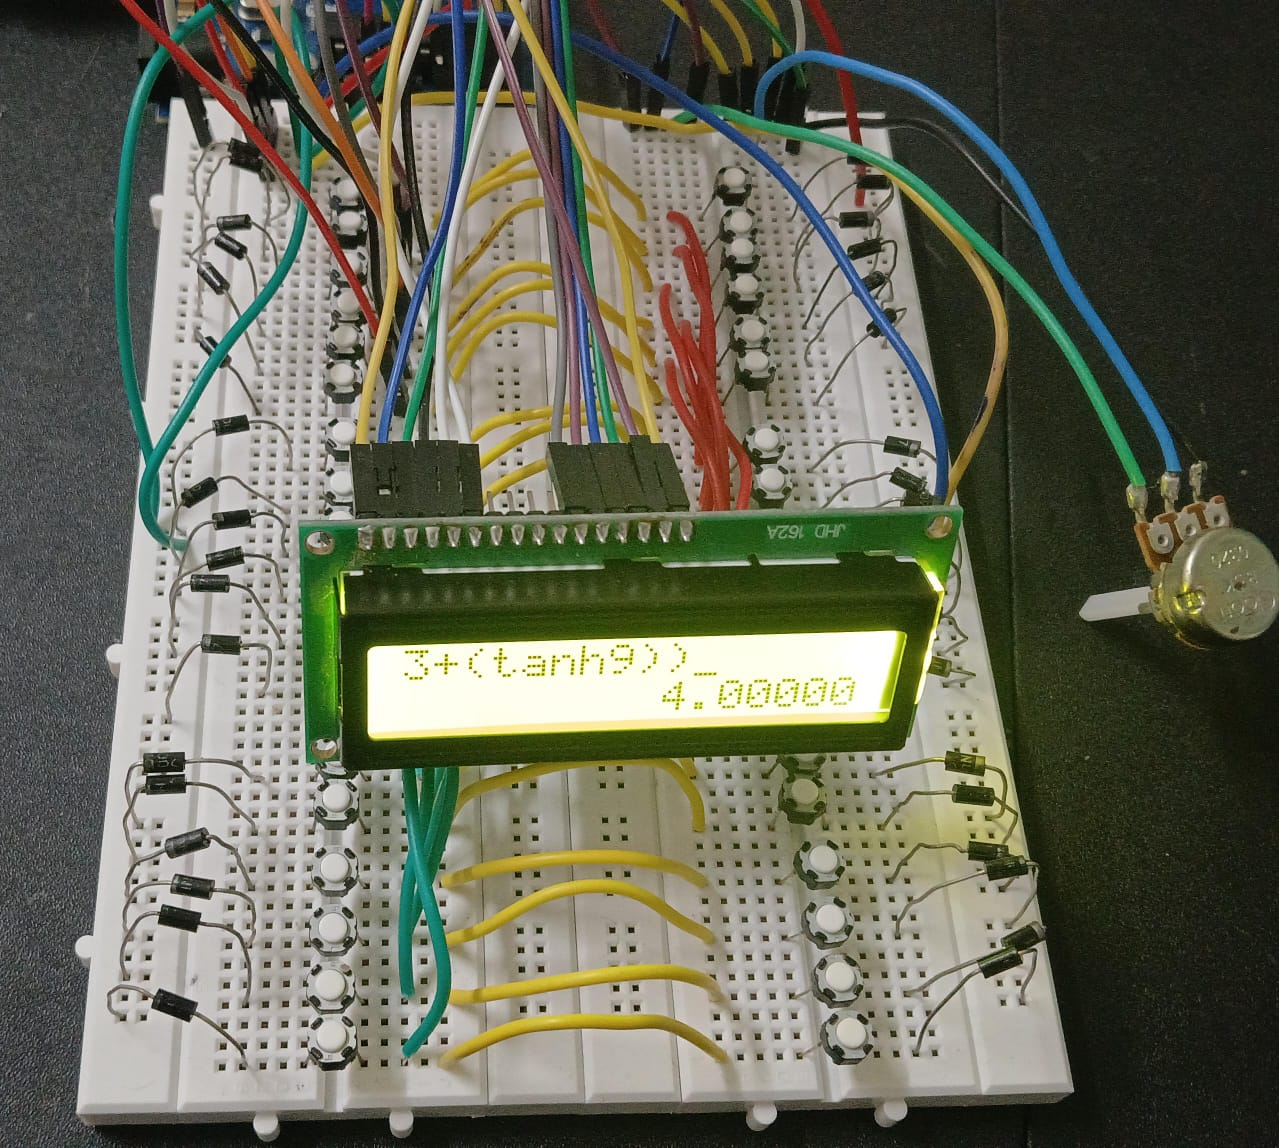
\includegraphics[width=0.9\linewidth]{figs/Cal.jpeg}
    \caption{Calculator}
    \label{fig:enter-label}
\end{figure}
\newpage
\section{Mathematical Expressions}
\subsection{Core Trigonometric Functions}
\begin{itemize}
    \item $\sin(x)$, $\cos(x)$, $\tan(x)$ : Implemented using RK4 to solve the differential equation $y'' = -y$ with appropriate initial conditions. These provide the fundamental trigonometric operations.
\end{itemize}

\subsection{Inverse Trigonometric Functions}
\begin{itemize}
    \item $\arcsin(x)$, $\arccos(x)$, $\arctan(x)$ : Calculate inverse trigonometric functions using RK4 with their respective differential equations.
\end{itemize}

\subsection{Exponential and Logarithmic Functions}
\begin{itemize}
    \item $\text{pow}(x, w)$ : Power function using RK4 for $\frac{dy}{dx} = w\frac{y}{x}$
    \item $\ln(x)$ : Natural logarithm using RK4 for $\frac{dy}{dx} = \frac{1}{x}$
\end{itemize}

\subsection{Hyperbolic Functions}
\begin{itemize}
    \item $\sinh(x)$, $\cosh(x)$, $\tanh(x)$ : Hyperbolic functions implemented using the exponential definitions.
\end{itemize}

\subsection{Utility Functions}
\begin{itemize}
    \item $\text{fast\_inv\_sqrt}(x)$ : Fast inverse square root using the famous Quake III algorithm.
    \item $\text{principal\_range}(\theta)$ : Normalizes angles to $[0, 2\pi]$ range.
    \item $\text{factorial}(n)$ : Calculates factorial for non-negative integers.
    \item $\text{dtf}(\text{decimal}, *\text{numerator}, *\text{denominator})$ : Converts decimals to fractions.
\end{itemize}

\subsection{Mathematical Constants}
\begin{itemize}
    \item $\pi = 3.14159265358979323846$
    \item $e = 2.7182818284$
\end{itemize}

\subsection{Important Implementation Notes}
\begin{enumerate}
    \item The functions use a step size $H = 0.01$ for numerical approximation.
    \item Error handling is implemented for edge cases (negatives, zeros).
    \item The code uses $\text{fast\_inv\_sqrt}$ for optimization where appropriate.
\end{enumerate}

For a calculator implementation, these functions provide a complete set of mathematical operations covering:
\begin{itemize}
    \item Basic arithmetic (through $\text{pow}$)
    \item Trigonometry (standard and inverse functions)
    \item Exponential and logarithmic calculations
    \item Hyperbolic functions
    \item Number theory operations (GCD, factorial, decimal-to-fraction conversion)
\end{itemize}

The numerical approach using RK4 is particularly interesting as it solves the functions through differential equations rather than series expansions, potentially offering good performance for a wide range of inputs.

% \subsection{Code}
% {Code for functions}
% \lstset{
%         language = C,
%         basicstyle=\ttfamily\tiny,
%         keywordstyle=\color{blue},
%         stringstyle=\color{green},
%         commentstyle=\color{gray},
%         tabsize=4
%     }
% \lstinputlisting{./codes/funcs.c}

\subsection{Code-funcs.c}
\begin{lstlisting}

#include <stdint.h>

#define PI 3.14159265358979323846
#define H 0.01
#define MAX_ITERS 100000
#define E 2.7182818284

double fast_inv_sqrt(double x){
    if(x <= 0) return 0;
    x = (float) x;
	long i;
	float x2, y;
	const float threehalfs = 1.5F;

	x2 = x * 0.5F;
	y  = x;
	i  = * ( long * ) &y;
	i  = 0x5f3759df - ( i >> 1 );
	y  = * ( float * ) &i;
	y  = y * ( threehalfs - ( x2 * y * y ) );

	return (double) y;
}

double principal_range(double angle) {
    int k = (int)(angle / (2*PI));
    angle -= k * (2*PI);
    if (angle < 0) angle += (2*PI);
    return angle;
}

// Sine calculation using RK4 for y'' = -y
double sin(double x_target) {
    double x = 0.0;     // Start point
    double y = 0.0;     // y(0) = 0
    double dy = 1.0;    // y'(0) = 1

    double h = H;    // Step size
    int steps = (int)(x_target / h); // Number of steps

    for (int i = 0; i < steps; i++) {
        double k1_y = h * dy;
        double k1_dy = h * (-y);

        double k2_y = h * (dy + 0.5 * k1_dy);
        double k2_dy = h * (-(y + 0.5 * k1_y));

        double k3_y = h * (dy + 0.5 * k2_dy);
        double k3_dy = h * (-(y + 0.5 * k2_y));

        double k4_y = h * (dy + k3_dy);
        double k4_dy = h * (-(y + k3_y));

        y += (k1_y + 2 * k2_y + 2 * k3_y + k4_y) / 6.0;
        dy += (k1_dy + 2 * k2_dy + 2 * k3_dy + k4_dy) / 6.0;

        x += h;
    }

    return y; // Return y at x_target
}

double cos(double x_target) {
    double x = 0.0;     // Start point
    double y = 1.0;     // y(0) = 1
    double dy = 0.0;    // y'(0) = 0
    
    double h = H;    // Step size
    int steps = (int)(x_target / h); // Number of steps

    for (int i = 0; i < steps; i++) {
        double k1_y = h * dy;
        double k1_dy = h * (-y);

        double k2_y = h * (dy + 0.5 * k1_dy);
        double k2_dy = h * (-(y + 0.5 * k1_y));

        double k3_y = h * (dy + 0.5 * k2_dy);
        double k3_dy = h * (-(y + 0.5 * k2_y));

        double k4_y = h * (dy + k3_dy);
        double k4_dy = h * (-(y + k3_y));

        y += (k1_y + 2 * k2_y + 2 * k3_y + k4_y) / 6.0;
        dy += (k1_dy + 2 * k2_dy + 2 * k3_dy + k4_dy) / 6.0;

        x += h;
    }

    return y; // Return y at x_target
}

double tan(double x){
    return sin(x)/cos(x);
}

// Power function using RK4 for dy/dx = w*y/x
double pow(double x, double w) {
    if(x < 0 && ((int) w) != w) return 0;
    if (x == 0) return 0;
    if (w == 0) return 1;
    
    if(x < 0) return ( ((int) w)%2 == 0 ? 1: -1)*pow(-x, w);

    double x0 = 1.0, y = 1.0;
    double target = x;
    int steps = (int)((target - x0) / H);
    
    for (int i = 0; i < steps; i++) {
        double k1 = H * w * y / x0;
        double k2 = H * w * (y + k1/2) / (x0 + H/2);
        double k3 = H * w * (y + k2/2) / (x0 + H/2);
        double k4 = H * w * (y + k3) / (x0 + H);
        
        y += (k1 + 2*k2 + 2*k3 + k4) / 6;
        x0 += H;
    }
    
    return y;
}

// Natural log using RK4 for dy/dx = 1/x
double ln(double x) {
    if (x <= 0) return 0.0;
    if (x < 1) return -ln(1/x);
    
    double x0 = 1.0, y = 0.0;
    int steps = (int)((x - x0) / H);
    
    for (int i = 0; i < steps; i++) {
        double k1 = H / x0;
        double k2 = H / (x0 + H/2);
        double k3 = H / (x0 + H/2);
        double k4 = H / (x0 + H);
        
        y += (k1 + 2*k2 + 2*k3 + k4) / 6;
        x0 += H;
    }
    
    return y;
}

double arctan(double x) {
    double x0 = 0.0, y = 0.0;
    int steps = x >= 0 ? (int) (x / H): (int) (-x / H); 
    double step_dir = (x >= 0) ? 1 : -1;
    
    for (int i = 0; i < steps; i++) {
        double k1 = H / (1 + x0*x0);
        double k2 = H / (1 + (x0 + H/2)*(x0 + H/2));
        double k3 = H / (1 + (x0 + H/2)*(x0 + H/2));
        double k4 = H / (1 + (x0 + H)*(x0 + H));
        
        y += step_dir * (k1 + 2*k2 + 2*k3 + k4) / 6;
        x0 += step_dir * H;
    }
    
    return y;
}

double arcsin(double x) {
    if (x < -1 || x > 1) return 0;

    double x0 = 0.0, y = 0.0;
    int steps = x >= 0 ? (int) (x / H): (int) (-x / H); 
    double step_dir = (x >= 0) ? 1 : -1;

    for (int i = 0; i < steps; i++) {
        double k1 = H * fast_inv_sqrt(1 - x0*x0);
        double k2 = H * fast_inv_sqrt(1 - (x0 + step_dir*H/2)*(x0 + step_dir*H/2));
        double k3 = H * fast_inv_sqrt(1 - (x0 + step_dir*H/2)*(x0 + step_dir*H/2));
        double k4 = H * fast_inv_sqrt(1 - (x0 + step_dir*H)*(x0 + step_dir*H));

        y += step_dir * (k1 + 2*k2 + 2*k3 + k4) / 6;
        x0 += step_dir * H;
    }

    return y;
}

double arccos(double x){
    return ((PI/2) - arcsin(x));
}

double factorial(double n) {
    if(n < 0) return 0;
    if(n == 0 || n == 1) return 1;

    double result = 1.0;
    
    for(double i = (int) n; i >= 2 ; i--) {
        result *= i;
    }
    
    return result;
}

int gcd(int a, int b) {
    int temp;

    while (b != 0) {
        temp = b;
        b = a % b;
        a = temp;
    }

    return a;
}

void dtf(double decimal, long int* numerator, long int* denominator) {
    *numerator = (int)(decimal * 1000000);
    *denominator = 1000000;
    
    int gcd_ = gcd(*numerator, *denominator);
    
    *numerator = *numerator/gcd_;
    *denominator = *denominator/gcd_;
}

double sinh(double x) {
    return (pow(E, x) - pow(E, -x)) / 2;
}

double cosh(double x) {
    return (pow(E, x) + pow(E, -x)) / 2;
}

double tanh(double x) {
    return sinh(x) / cosh(x);
}


\end{lstlisting}
\section{Overall System Architecture}
The embedded calculator is implemented on an AVR microcontroller and consists of three main components:

\begin{itemize}
    \item Expression Parsing and Evaluation System
    \item User Interface and Input Handling
    \item Hardware Interaction Layer
\end{itemize}
\section{Expression Parsing and Evaluation System}

\subsection{Key Data Structures}

The token structure represents different types of mathematical elements:

\begin{lstlisting}[caption=Token Structure, label=lst:token]
typedef struct Token {
    TokenType type;     // Type of token (number, operator, function)
    TokenVal val;       // Value of the token
} Token;
\end{lstlisting}
\subsection{Shunting Yard Algorithm for Parsing}
The calculator uses the Shunting Yard algorithm to convert infix expressions to Reverse Polish Notation (RPN). This algorithm ensures operator precedence and left-to-right evaluation.

The algorithm is implemented as follows:

\begin{lstlisting}[caption=Shunting Yard Algorithm Implementation, label=lst:shuntingyard]
void processTokens(Token token_stream[], short size, Token output_stack[], short *output_size, Token operator_stack[], short *operator_size) {
    for (int i = 0; i < size; i++) {
        Token token = token_stream[i];
        
        if (token.type == NUM) {
            append(output_stack, output_size, token);
        } else if (token.type == OP) {
            while (*operator_size > 0 && precedence(token.val.op) <= precedence(operator_stack[*operator_size - 1].val.op)) {
                append(output_stack, output_size, pop(operator_stack, operator_size));
            }
            append(operator_stack, operator_size, token);
        } else if (token.type == LBRAK) {
            append(operator_stack, operator_size, token);
        } else if (token.type == RBRAK) {
            while (*operator_size > 0 && operator_stack[*operator_size - 1].type != LBRAK) {
                append(output_stack, output_size, pop(operator_stack, operator_size));
            }
            pop(operator_stack, operator_size); // Remove left bracket
        }
    }
    
    while (*operator_size > 0) {
        append(output_stack, output_size, pop(operator_stack, operator_size));
    }
}
\end{lstlisting}

\subsection{Evaluation of RPN Expressions}

Once the expression is converted to RPN, it is evaluated using a stack-based approach.

\begin{lstlisting}[caption=RPN Evaluation, label=lst:rpneval]
double evaluateRPN(Token output_stack[], short output_size, double ans) {
    Token res_stack[STACK_SIZE];
    short res_size = 0;
    
    for (int i = 0; i < output_size; i++) {
        Token token = output_stack[i];
        
        if (token.type == NUM) {
            append(res_stack, &res_size, token);
        } else if (token.type == OP) {
            Token right = pop(res_stack, &res_size);
            Token left = pop(res_stack, &res_size);
            Token res_token;
            res_token.type = NUM;
            
            switch (token.val.op) {
                case ADD: res_token.val.num = left.val.num + right.val.num; break;
                case SUB: res_token.val.num = left.val.num - right.val.num; break;
                case MUL: res_token.val.num = left.val.num * right.val.num; break;
                case DIV: res_token.val.num = left.val.num / right.val.num; break;
                case POW: res_token.val.num = pow(left.val.num, right.val.num); break;
            }
            append(res_stack, &res_size, res_token);
        }
    }
    return res_stack[0].val.num;
}
\end{lstlisting}

\textbf{Remark:}
 Button matrix implementation and operator precedence are sourced from EE24BTECH11002 - $Agamjot \,\, Singh$\\
 
 link:-\href{https://github.com/agamjotsingh1/EE1003/tree/main/hardware/embedded_c/calci}{hyperlink}
\newpage
\section{User Interface and Input Handling}

\subsection{Input Mechanisms}

The calculator employs a 6x6 matrix keypad with the following features:

\begin{itemize}
    \item Mode switching capability
    \item Button debouncing mechanism
    \item Two button mapping arrays for Standard and Advanced modes
\end{itemize}

The keypad handling function is implemented as follows:

\begin{lstlisting}[caption=Keypad Input Handling, label=lst:keypad]
char getKeypadInput() {
    for (int row = 0; row < ROWS; row++) {
        for (int col = 0; col < COLS; col++) {
            if (isButtonPressed(row, col)) {
                return keyMap[row][col];
            }
        }
    }
    return '\0';
}
\end{lstlisting}

\subsection{Button Matrix Scanning and Debouncing}

A button matrix scanning mechanism ensures accurate key detection. The process involves:

\begin{itemize}
    \item Setting each row LOW sequentially
    \item Reading column states to detect key presses
    \item Implementing software debouncing for stable key readings
\end{itemize}

The button matrix scanning function is implemented as follows:

\begin{lstlisting}[caption=Button Matrix Scanning, label=lst:buttonmatrix]
void scanButtonMatrix() {
    for (int row = 0; row < ROWS; row++) {
        setRowLow(row);
        
        for (int col = 0; col < COLS; col++) {
            if (readColumn(col) == LOW) {
                debounceButton(row, col);
            }
        }
        
        setRowHigh(row);
    }
}
\end{lstlisting}

\subsection{Debouncing Mechanism}

Debouncing prevents multiple unwanted detections from a single press:

\begin{lstlisting}[caption=Debounce Function, label=lst:debounce]
void debounceButton(int row, int col) {
    _delay_ms(DEBOUNCE_TIME);
    if (readColumn(col) == LOW) {
        registerKeyPress(row, col);
    }
}
\end{lstlisting}

\subsection{Display Management}

The LCD display:

\begin{itemize}
    \item Supports a 16x2 character display
    \item Handles multi-line expressions
    \item Converts abbreviated function names to full names
    \item Manages scrolling for long expressions
\end{itemize}

\section{Hardware Interaction Layer}

\subsection{Memory Management}

\begin{itemize}
    \item Uses EEPROM for persistent storage
    \item Supports memory recall and storage operations
    \item Employs optimized memory management using fixed-size buffers
\end{itemize}

The EEPROM read function is shown below:

\begin{lstlisting}[caption=EEPROM Read Function, label=lst:eeprom]
uint8_t readEEPROM(uint16_t address) {
    while (EECR & (1 << EEPE)); // Wait for completion
    EEAR = address;
    EECR |= (1 << EERE);
    return EEDR;
}
\end{lstlisting}

\subsection{Microcontroller Interfaces}

\begin{itemize}
    \item Direct port manipulation for LCD and keypad
    \item Uses AVR-specific libraries and macros
    \item Minimizes dynamic memory allocation
\end{itemize}

\section{Optimization Strategies}

\subsection{Memory Optimization}

\begin{itemize}
    \item Fixed-size statically allocated arrays
    \item Minimal dynamic memory usage
    \item Efficient bit manipulation macros
    \item Compact token representation using a union
\end{itemize}

\subsection{Performance Optimization}

\begin{itemize}
    \item Efficient parsing algorithm
    \item Minimal computational overhead
    \item Direct hardware register manipulation
    \item Predefined constants for repeated calculations
\end{itemize}

\section{Key Design Patterns}

The software architecture employs:

\begin{itemize}
    \item \textbf{State Machine}: Used for button handling
    \item \textbf{Interpreter Pattern}: Applied in expression evaluation
    \item \textbf{Command Pattern}: Used for button mapping
\end{itemize}

\section{Potential Improvements}

Future enhancements may include:

\begin{itemize}
    \item Advanced error handling for complex expressions
    \item Additional mathematical functions
    \item Improved memory management
    \item Enhanced floating-point precision handling
\end{itemize}

\end{document}

